\chapter[SCP-017 影魔]{
    SCP-017 Shadow Person\\
    SCP-017 影魔
}

\label{chap:SCP-017}

\begin{figure}[H]
    \centering
    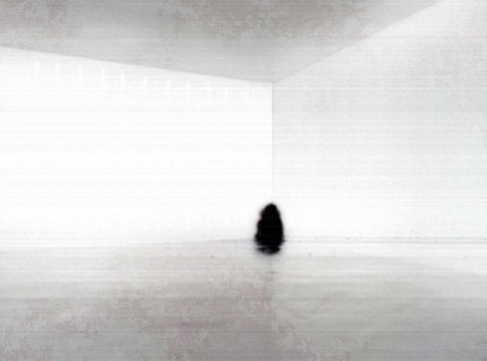
\includegraphics[width=0.5\linewidth]{images/SCP.017.jpg}
    \caption*{SCP-017档案相片}
\end{figure}

\bb{项目编号:}SCP-017

\bb{项目等级:}Keter

\bb{特殊收容措施:}SCP-017保存于一个大小为6米 X 6米 X 4米的房间,悬浮于正中央一个100厘米 X 50厘米 X 50厘米的丙烯酸玻璃牢笼内。此房间的墙壁,天花板和地板都布满弧光照明灯,对准正中的笼子,以确保SCP-017时刻暴露于所有角度的光照下。进入SCP-017控制室的指定人员只进行下列工作:检测聚光灯和临时发电器功能,一旦发现灯泡烧坏或者发电机出现故障,立即请求维护。

只有在需要更换灯泡的唯一情况下允许工作人员进入房间内。进入房间的工作人员需要穿着特制的全反光制服,且需绝对谨慎,不能挡在任何正常工作的灯泡前。

\bb{描述:}SCP-017具有人形轮廓,高80厘米,外形类似于人类幼童,但没有任何可辨别的外貌特征。SCP-017身体似乎由一团模糊不清的烟幕组成。烟幕内部至今没有成功发现过任何实体物质,但不能完全排除在未来发现的可能性。

一旦有影子产生且覆盖于SCP-017上,SCP-017会迅速产生反应。它会立刻将影子来源整个包裹进烟幕之中,然后烟幕会变回通常大小。被包裹对象就此消失得无影无踪。

\bb{备注:}具有BETA或更高权限的工作人员获准查看档案\#017-1。
